% Document principal LaTeX pour compte-rendu
\documentclass[12pt]{report}
\usepackage{BidoTexCourses}
\usepackage{hyperref}
\usepackage{graphicx}


\title{Compte rendu projet Portal 0.0}
\author{BIDAULT Matthieu, BADSTÜBER Elian, FOCHEUX Vital}
\date{\today}

\renewcommand{\contentsname}{
	Table des matières
}

\begin{document}

\maketitle

\section*{Remerciements}

Nous tenons à remercier notre enseignant de projet, M. \textsc{Bernard} 
qui a su nous guider et nous conseiller tout au long de ce projet.


\tableofcontents

\section{Introduction}

Dans le cadre du projet semestriel de troisième année de licence
informatique à l'université de Franche-Comté, nous proposons de coder
une version très simplifiée du jeu \href{https://fr.wikipedia.org/wiki/Portal_(jeu_vid%C3%A9o)}{Portal}
qui sera afficher grâce à un moteur de type Raycaster à la façon du jeu
\href{https://fr.wikipedia.org/wiki/Wolfenstein_3D}{Wolfenstein 3D}.
Il a pour but de nous faire découvrir le monde du développement de jeux 
vidéo en nous faisant réaliser un jeu vidéo en C++ avec la bibliothèque 
\href{https://gamedevframework.github.io/}{Gamedev Framework} (GF)\footnote{Tous au long de ce rapport, nous utiliserons abbrévation GF.
Cela signifie Gamedev Framework.}.


\section{Besoins et objectifs du projet}
\subsection{Contexte}

\begin{figure}
	\begin{minipage}{0.48\textwidth}
		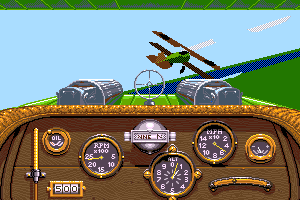
\includegraphics[width=\linewidth]{image/knights-of-the-sky.png}
		\hspace*{-0.5cm}
		\caption{Knights of the Sky}
		\label{fig:knights-of-the-sky}
	\end{minipage}
	\begin{minipage}{0.48\textwidth}
		\centering
		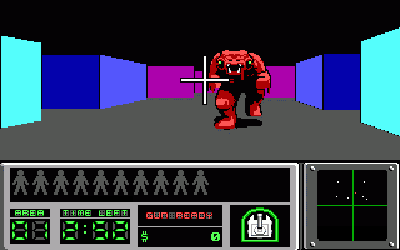
\includegraphics[width=\linewidth]{image/Hovertank_3D.png}
		\hspace*{-0.5cm}
		\caption{Hovertank 3D}
		\label{fig:hovertank3d}
	\end{minipage}
\end{figure}

\begin{figure}
	\begin{minipage}{0.48\textwidth}
		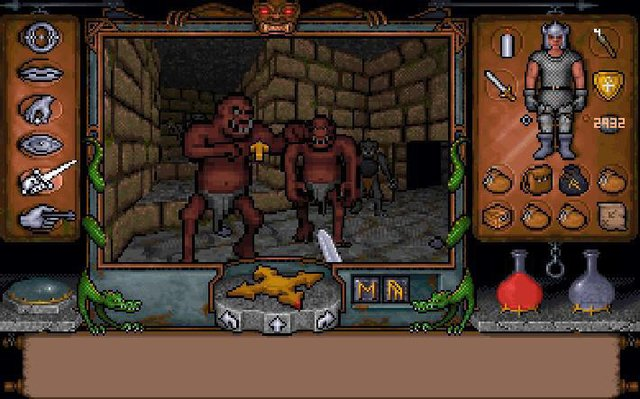
\includegraphics[width=\linewidth]{image/Ultima_Underworld.jpg}
		\hspace*{-0.5cm}
		\caption{Ultima Underworld}
		\label{fig:ultimaunderworld}
	\end{minipage}
	\begin{minipage}{0.48\textwidth}
		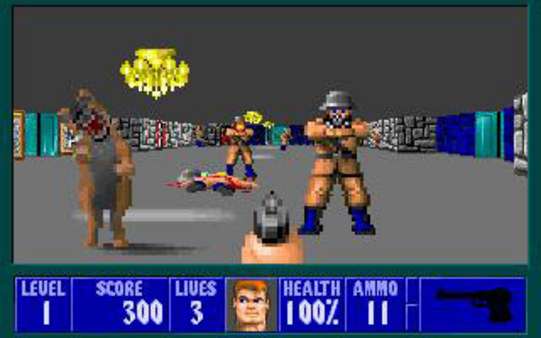
\includegraphics[width=\linewidth]{image/wolfenstein_3d.jpg}
		\hspace*{-0.5cm}
		\caption{Wolfenstein 3D}
		\label{fig:wolfenstein3d}
	\end{minipage}
\end{figure}

\paragraph{Les graphismes :}
Au début des années 90, la société \href{https://fr.wikipedia.org/wiki/Id_Software}{Id Software} a entrepris des 
recherches pionnières dans le domaine des graphismes 3D, alors principalement réservés aux simulateurs de vols tels 
que \href{https://fr.wikipedia.org/wiki/Wing_Commander_(jeu_vid%C3%A9o)}{Wing Commander} ou 
\href{https://en.wikipedia.org/wiki/Knights_of_the_Sky}{Knights of the Sky} (\nameref{fig:knights-of-the-sky}), deux titres parus en 1990. Face aux 
contraintes de performance des ordinateurs de l'époque, le développement de jeux d'action en 3D rapide représentait 
un défi de taille. C'est dans ce contexte que \href{https://fr.wikipedia.org/wiki/John_Carmack}{John Carmack} a 
proposé l'utilisation de la technique du \href{https://fr.wikipedia.org/wiki/Raycasting}{raycasting}, permettant 
de calculer uniquement les surfaces visibles par le joueur. En six semaines, Carmack développe un moteur 3D innovant 
utilisant des sprites 2D pour représenter les entités du jeu. Ce moteur a été utilisé dans le jeu 
\href{https://fr.wikipedia.org/wiki/Hovertank_3D}{Hovertank 3D} (\nameref{fig:hovertank3d}), publié en avril 1991.
À l'automne 1991, alors que \href{https://fr.wikipedia.org/wiki/John_Carmack}{John Carmack} et 
\href{https://fr.wikipedia.org/wiki/John_Romero}{John Romero} finalisaient le moteur de 
\href{https://en.wikipedia.org/wiki/Commander_Keen_in_Goodbye,_Galaxy}{Commander Keen in Goodbye, Galaxy}, Carmack 
découvre \href{https://fr.wikipedia.org/wiki/Ultima_Underworld}{Ultima Underworld} (\nameref{fig:ultimaunderworld}), un jeu développé par 
\href{https://fr.wikipedia.org/wiki/Looking_Glass_Studios}{Blue Sky Productions} (qui deviendra plus tard Looking Glass Studios), 
doté d'un moteur capable de rendre des graphismes 3D texturés sans subir les limitations de Hovertank 3D.
Inspiré, Carmack décide d'améliorer son propre moteur pour 
intégrer le mapping de textures tout en conservant de hautes performances. Après un intense travail de six semaines, 
le nouveau moteur 3D est achevé et utilisé pour le jeu \href{https://fr.wikipedia.org/wiki/Catacomb_3D}{Catacomb 3D},
publié en novembre 1991. La révélation de Catacomb 3D a poussé 
\href{https://fr.wikipedia.org/wiki/Scott_Miller_(programmeur)}{Scott Miller} d'Apogee à convaincre l'équipe de 
développer un jeu d'action en 3D sous forme de shareware. Cela a conduit au lancement du projet 
\href{https://fr.wikipedia.org/wiki/Wolfenstein_3D}{Wolfenstein 3D} (\nameref{fig:wolfenstein3d}), un remake en 3D de 
\href{https://fr.wikipedia.org/wiki/Castle_Wolfenstein}{Castle Wolfenstein}. Sorti le 5 mai 1992 sur PC, ce jeu a 
non seulement été un succès commercial mais a également posé les bases du genre du jeu de tir à la première personne, 
préfigurant ainsi des titres légendaires tels que 
\href{https://fr.wikipedia.org/wiki/Doom_(jeu_vid%C3%A9o,_1993)}{Doom} et 
\href{https://fr.wikipedia.org/wiki/Quake}{Quake}.

\begin{figure}
	\centering
	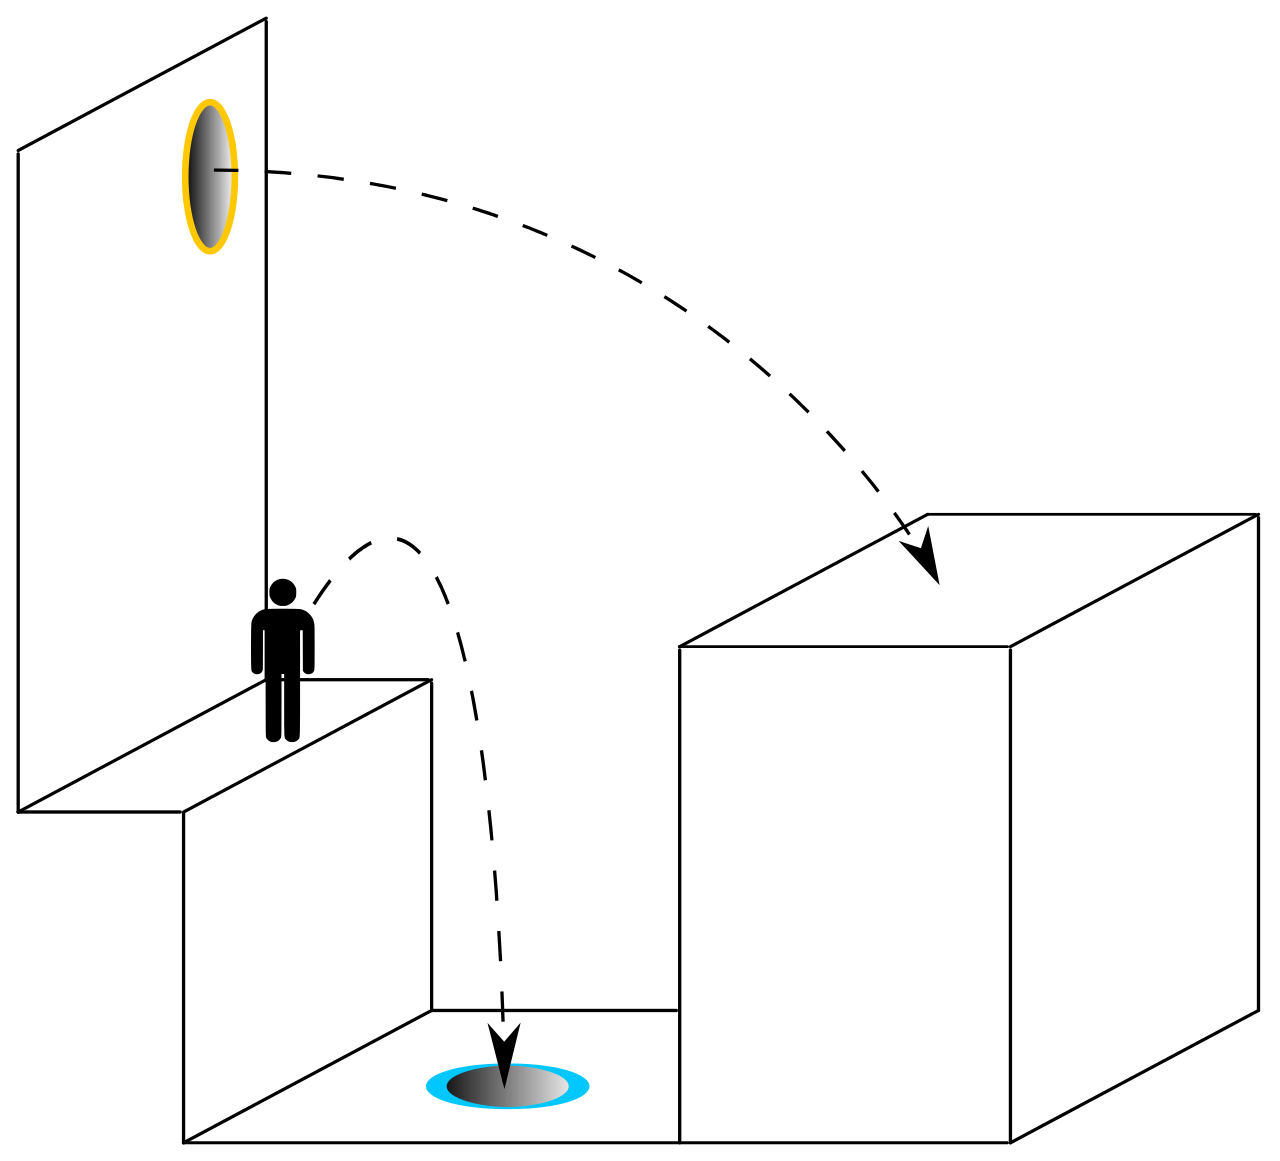
\includegraphics[width=0.5\textwidth]{image/schema_portal.png}
	\hspace*{-0.5cm}
	\caption{Schéma de fonctionnement du système de portail}
	\label{fig:schema_portal}
\end{figure}

\paragraph{Le système de jeu : }
En 2007, \href{https://fr.wikipedia.org/wiki/Valve_Corporation}{Valve Corporation} a révolutionné le genre des jeux 
de réflexion à la première personne avec la sortie de 
\href{https://fr.wikipedia.org/wiki/Portal_(jeu_vid%C3%A9o)}{Portal}. Ce jeu introduit un mécanisme unique 
permettant au joueur de générer deux portails, l'un orange et l'autre bleu, sur des surfaces planes et 
interconnectées. Ces portails offrent la possibilité de traverser instantanément l'espace d'un point à un autre, 
tout en conservant l'inertie. L'objectif est de résoudre divers puzzles en se servant de cette capacité à manipuler 
l'espace pour atteindre la sortie des différents niveaux proposés.



\subsection{Motivations}


L'une des motivations principales de ce projet est de réaliser un jeu vidéo
avec graphique comme à l'époque de \href{https://fr.wikipedia.org/wiki/Wolfenstein_3D}{Wolfenstein 3D} 
mais avec des comcepts de jeux plus récentes et qui plus est pourrai être
un préquel de \href{https://fr.wikipedia.org/wiki/Portal_(jeu_vid%C3%A9o)}{Portal}.


\subsection{Objectif et contraintes}

Les principaux objectifs de ce projet sont :
\begin{itemize}
	\item Réaliser un jeu vidéo en C++ avec la bibliothèque GF
	\item Implémenter un moteur de type Raycaster
	\item Implémenter un système de portail
	\item Implémenter un système de collision
	\item Offir une expérience de jeu simple et agréable à jouer.
\end{itemize}

Mais avec des contraintes :
\begin{itemize}
	\item L'apprentissage d'un langage de programmation nouveau pour nous
	\item L'apprentissage d'une bibliothèque de programmation nouvelle pour nous
	\item L'apprentissage de la programmation d'un moteur de type Raycaster
	\item L'apprentissage de la programmation d'un système de portail
	\item L'apprentissage de la programmation d'un système de collision
	\item L'apprentissage de la programmation d'un système de jeu
\end{itemize}

\section{Gestion du projet}
\subsection{L'équipe}
\subsection{Planification et outils de gestion}

Pour la gestion du projet nous avons utilisé le site 
\href{https://github.com/}{github} qui est un outil de gestion 
de projet en ligne.

\subsection{Répartition des tâches}

\section{Développement}
\subsection{Programmer en C++}

Programmer en C++ a pu s'avérer assez techniques car cela était un tout nouveau
langage de programmation à apprendre pour nous car il n'avait jamais été abordé
auparavant lors de notre parcours universitaire.

\subsection{Apprendre à utiliser la bibliothèque GF}

Une des plus grandes difficultés de ce projet était de développé avec la bibliothèque
GF. En effet, quand bien même c'est un bibliothèque possèdant un bon nombre de 
fonctions pouvant permettre le développement graphique 2D. Elle reste néanmoins
parfois limité pour les besoins techniques du projet, mais grâce à cela, cela permet
de donner des idées de méthodes à rajouter dans GF voire dans GF2.\footnote{GF2 est un projet
qui est la suite de GF en C++ ainsi qu'en python3.}


\subsection{Différentes stratégie}
\subsubsection{Première approche}

Une première approche du projet a d'abord été envisagée. Elle consistait 
basiquement à envoyer plus de rayons possibles à partir de la vision du joueur
afin de permettre le rendu des entités ainsi que des textures.

Cette approche étant facile et simpliste à implémenter une nouvelle approche
du projet a été prise en compte.

\subsubsection{Seconde approche plus technique}

Cette nouvelle approche de nôtre projet repose sur quelques même principe que
la première mais tout en étant plus technique sur le plan mathématiques et informatique.

\subsection{Détails du développement}

Dans cette partie nous allons détailler les différentes étapes de développement
de notre projet avec la seconde approche. En commencençant par la partie la 
moins technique pour finir par la partie la plus technique.
Il faut noté que détails du développement dans les parties qui vont suivre
sont pour un rendu 3D, mais tout au long de ce projet les différentes étapes
ont été tester sur un rendu 2D pour faciliter le développement.

\subsubsection{Les maps:}
Afin de pouvoir afficher des maps\footnote{En français les cartes}, 
nous avons dû créer un fichier PNG\footnote{Portable Network Graphics} où
nous dessinons les murs ainsi que la case de départ et d'arrivée. (insérer image ou schéma map)
Lors du lancement du jeu, le programme lit le fichier PNG et enregistre les
différentes cases dans un tableau à deux dimensions. En même temps, le programme
va regarder si les coordonnées correspondent à une cellule de mur, la case 
de départ, la case d'arrivée ou aucune des deux. Si c'est une cellule de mur, 
alors on va effectuer un parcours en profondeur des coordonnées adjacentes 
pour savoir si ceux sont des cellules de murs ou non. Grâce à cela nous 
pouvons récuperer toutes les cellules d'un mur directement et ainsi compter 
le nombre de mur assez facilement.

\subsubsection{Les murs:}

Dans cette partie nous allons détaillés les différentes étapes pour la création
des murs.

\paragraph{Récupération des sommets utiles:}

Pour la création des murs, on effectue un boucle sur la liste de coordonnées
des cellules occupées pour un mur précédemment récupérée. Sur chacune des 
coordonnées, on va regarder quatre de ses coordonnées adjacentes qui sont celles
en haut, en bas, à gauche et à droite. Si l'une d'entre elles fait partie de 
la liste des coordonnées des cellules alors on va incrémenter un compteur.
Si ce compteur est égal à 1 ou 3 alors on va l'ajouter dans une liste de coordonnées
dites utiles, c'est-à-dire que ceux sont les coordonnées des sommets des murs.

\paragraph{Triage des sommets:}
Afin de faciliter le rendu des murs, nous avons besoin de trier les sommets.
Pour cela, nous effectuons un boucle tant que la taille de la liste des 
sommets utiles est supérieur à la taille de la liste des sommets triés.
Dans cette boucle, nous allons effectuer une boucle sur la liste des sommets
utiles si le sommet est dans la liste des sommets triés ou non. Si il ne l'est
pas alors on va récupérer les coordonnées de ce sommet et faire appel à une fonction
pour trier à partir de ce sommet, la liste des sommets utiles et la liste des sommets
triés.
Dans cette fonction, on va effectuer une boucle sur la liste des sommets utiles
à partir du sommets donné en paramètre. On va regarder pour chaque sommet si il
existe un sommet dans la direction choisie ainsi que dans sa direction opposée.
(Explication de la fonction fctCanGo?)
\begin{itemize}
	\item Si il existe un sommet dans la direction choisie et aucun sommet dans
	la direction opposée alors on va ajouter ce sommet dans la liste des sommets
	triés.
	\item Sinon si il existe un sommet dans la direction opposée et aucun sommet
	dans la direction choisie alors on va ajouter le sommet de la direction opposée
	dans la liste des sommets triés et changer la direction courante par la 
	direction opposée.
	\item Sinon 
	\begin{itemize}
		\item Si il existe un sommet dans la direction choisie et un sommet 
		dans la direction opposée alors on regarder si le sommet de la 
		direction opposée n'est pas dans la liste des sommets triés et qu'un
		changement de direction doit être effectué ou bien que le sommet de 
		la direction choisie est dans la liste des sommets triés et qu'un 
		chanegement de direction ne doit pas être effectué alors on va ajouter
		le sommet de la direction opposée dans la liste des sommets triés
		et changer la direction courante par la direction opposée.
		\item Sinon on va ajouter le sommet de la direction choisie dans la liste 
		des sommets triés.
	\end{itemize}	
\end{itemize}
On va changer de direction en fonction de la direction courante, si le changement
de direction reste le même que l'ancien alors on va changer de direction.
Si n'existe aucune sommet dans les directions choisies et opposées alors on
va incrémenter un compteur. Si ce compteur est supérieur ou égal à 4 alors 
on arrête la fonction de triage.

\paragraph{Contruction des murs:}
Une fois les sommets utiles triés nous allons pouvoir construire les murs et
les ajouter dans une liste de murs. Chaque murs de cette liste a pour attributs
les coordonnées de ses sommets triés, les coordonnées de ses cellules occupées et
la taille de son périmètre.

\subsubsection{La boucle de jeu:}
Dans cette partie nous allons détailler les différentes étapes de la boucle de jeu.

\paragraph{Events:}
Nous allons tous d'abord gérer la gestion des évènements. 
Pour cela nous allons effectuer une boucle sur les évènements et pour chaque
bouton sur lesquels nous avons ajouté une action, nous allons effectuer cette
action. Nous allons aussi gérer les fonctions de déplacement de la vision 
grâce à la souris avec la position relative de la souris. Ensuite, nous allons
gérer la fonction d'envoie des portails en fonction du clic de la souris effectuer.

\paragraph{Update:}
Nous allons effectuer une update du jeu par rapport au temps écoulé depuis le
dernier update. Cette update va permettre de mettre à jour (les attributs du 
joueur). De calculer la nouvelle position du joueur si il est en colision avec 
un mur. Et enfin calculer les nouveaux attributs du joueur si il est proche d'un
portail lorsque les deux portails sont activés.

\paragraph{Render:}
Avant de faire le nouveau rendu des entités, nous allons d'abord effacer 
tous les rendus précédents. Enuiste nous allons effectuer le rendu de toutes
les entités que nous allons détaillés dans la parties suivante.

\subsubsection{Les renders:}
Ici explication de chaque rendu des différentes entités

\paragraph{Le rendu des murs:}
Pour le rendu des murs, nous allons effectuer une boucle sur la liste des sommets
triés. Pour chaque sommet, nous allons dessiner une ligne blanche entre le sommet
suivant dans la liste des sommets triés et le sommet courant. Si nous sommes à
la fin de la liste des sommets triés alors nous allons dessiner une ligne blanche
entre le sommet courant et le premier sommet de la liste des sommets triés.

\subsubsection{Les collisions:}

Explication des collisions avec les murs et les portails avec les schémas.


\section{Conclusion technique \& personnelle}
\subsection{Bilan du projet}
\subsubsection{Résultats obtenus}
\subsubsection{Apports technique}
\subsubsection{Apports personnels}

\subsection{Perspectives}
\subsubsection{Améliorations possibles}
\subsubsection{Nouvelles fonctionnalités}
\subsubsection{Un plus dans nos CV}

\section{Bibliographie}

Gamedev Framework (GF): \href{https://gamedevframework.github.io/}{https://gamedevframework.github.io/}


\end{document}